\section{Interpolation Methods}\label{background_interpolation_methods}
    This section focuses on the various statistical methods of interpolating and extrapolating data values at arbitrary points on a grid. These methods vary in their effectiveness on different data sets, however it is important to note that none of these methods take into account data which could be viewed as extremely important in this case. An example of this is the terrain. In section \todo{Fill in this reference} we discuss the effect that canyoning has on air quality readings. This effect is ignored by these models. 

    A further crucial piece of information which needs to be taken into account is that these models do not take into account temporal changes of readings. In order to use our data sets we will have to have a way of ``snapshotting'' data. A choice needs to be made for the length of time each snapshot should be. A suggestion for a rough value is 30 minutes, however experimental results will reveal the best value to use.

    With regards to the models chosen, various possibilities were considered. Due to the fact that various algorithms are similar with minor differences, the decision was made to use only a single algorithm from each ``family''. As such the algorithms chosen to be evaluated are:

    %http://en.wikipedia.org/wiki/Multivariate_interpolation
    \begin{itemize}
        \item Bicubic interpolation
        \item Natural neighbour interpolation
        \item Spline interpolation
        \item Nearest neighbour interpolation
        \item Inverse distance weighting interpolation
        \item Barnes interpolation
    \end{itemize}

    These algorithms can be split into two categories, regular grid algorithms and irregular grid algorithms, based on the format of the input data expected. 

    \subsection{Regular Grid Algorithms}\label{background_interpolation_methods_regulargrid}

        \tdi{This should be in the PredictionEvaluation Section}
        These interpolation methods require a regular grid with data points placed onto them and will calculate all missing values. In order to conform to this the data into ``buckets''. Buckets of area $100m^{2}$ will allow us to have a reasonable resolution for data without sacrificing calculation speed. The two furthest points of the Zurich tram network are roughly $5km$ apart and so we shall use a map which is the square of this distance, which results in a grid resolution of 500*500, for a total of 250,000 data points. 

        \subsubsection{Bicubic}\label{background_interpolation_methods_bicubic}

            Bicubic interpolation is the simplest of the grid interpolation algorithms which will be evaluated. As a cubic Hermite spline~\cite{practicalguidesplines} the output is smoother than linear interpolation methods such as bilinear interpolation, as we can see in figure~\ref{fig:bicubic_vs_bilinear}. The bicubic algorithm achieves this by taking into account the 16 points surrounding the point to be interpolated rather than just 4. 

            \begin{figure}[H]
                \centering
                \begin{subfigure}{.5\textwidth}
                    \centering
                    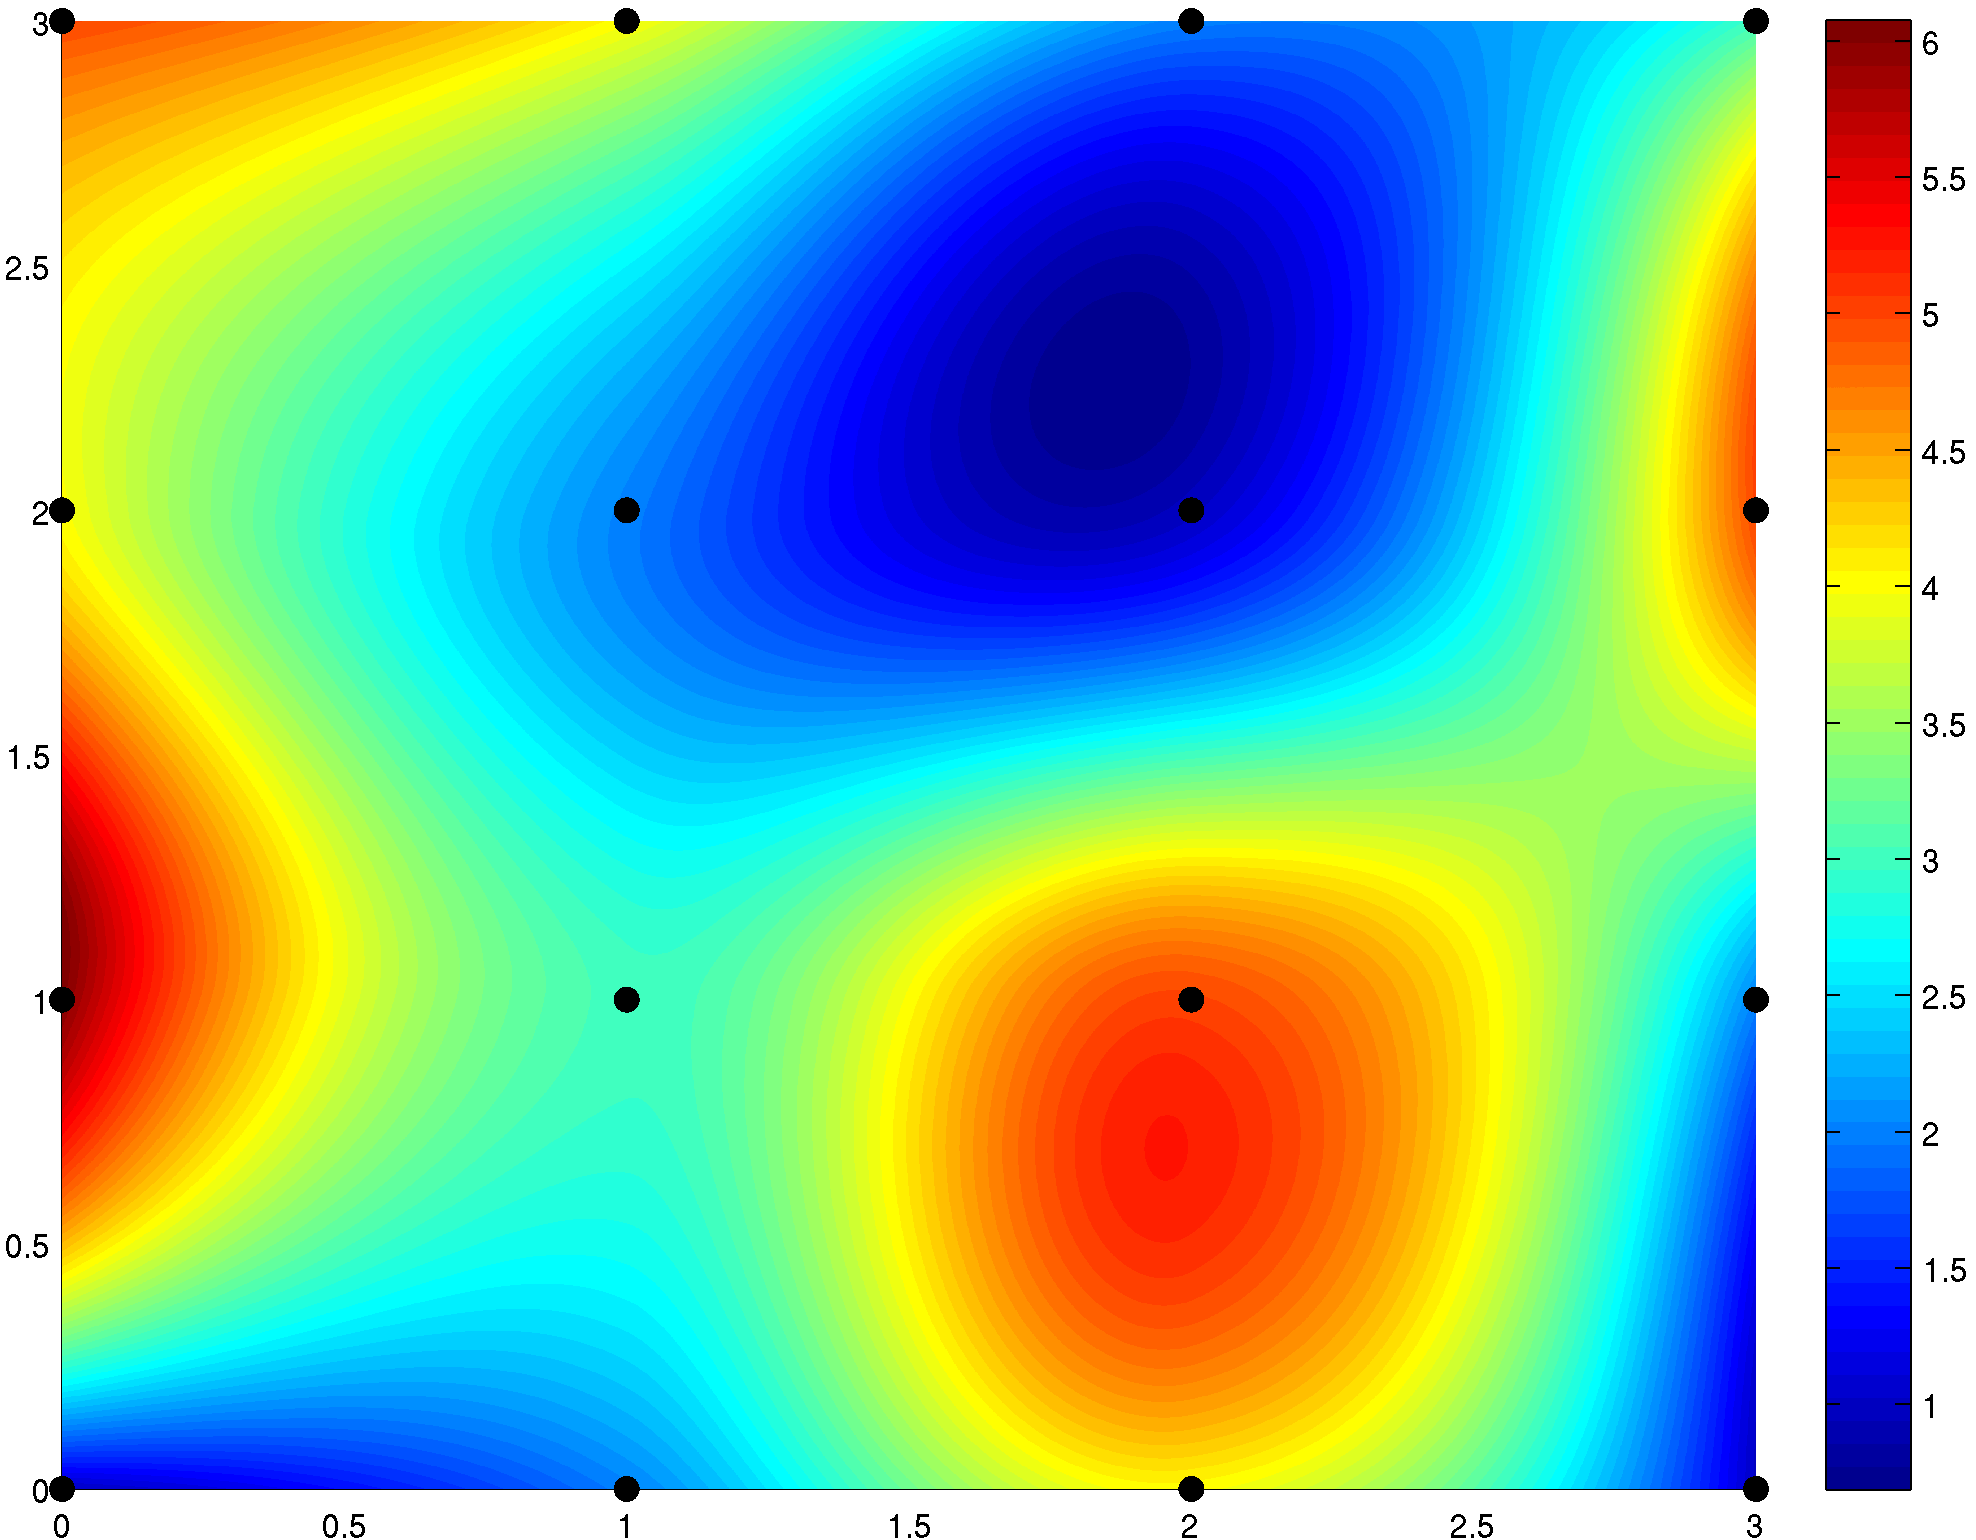
\includegraphics[width=0.9\linewidth]{./images/Bicubic_Interpolation_Example.png}
                    \caption{}
                    \label{fig:example_bicubic}
                \end{subfigure}%DO NOT REMOVE THIS COMMENT
                \begin{subfigure}{.5\textwidth}
                    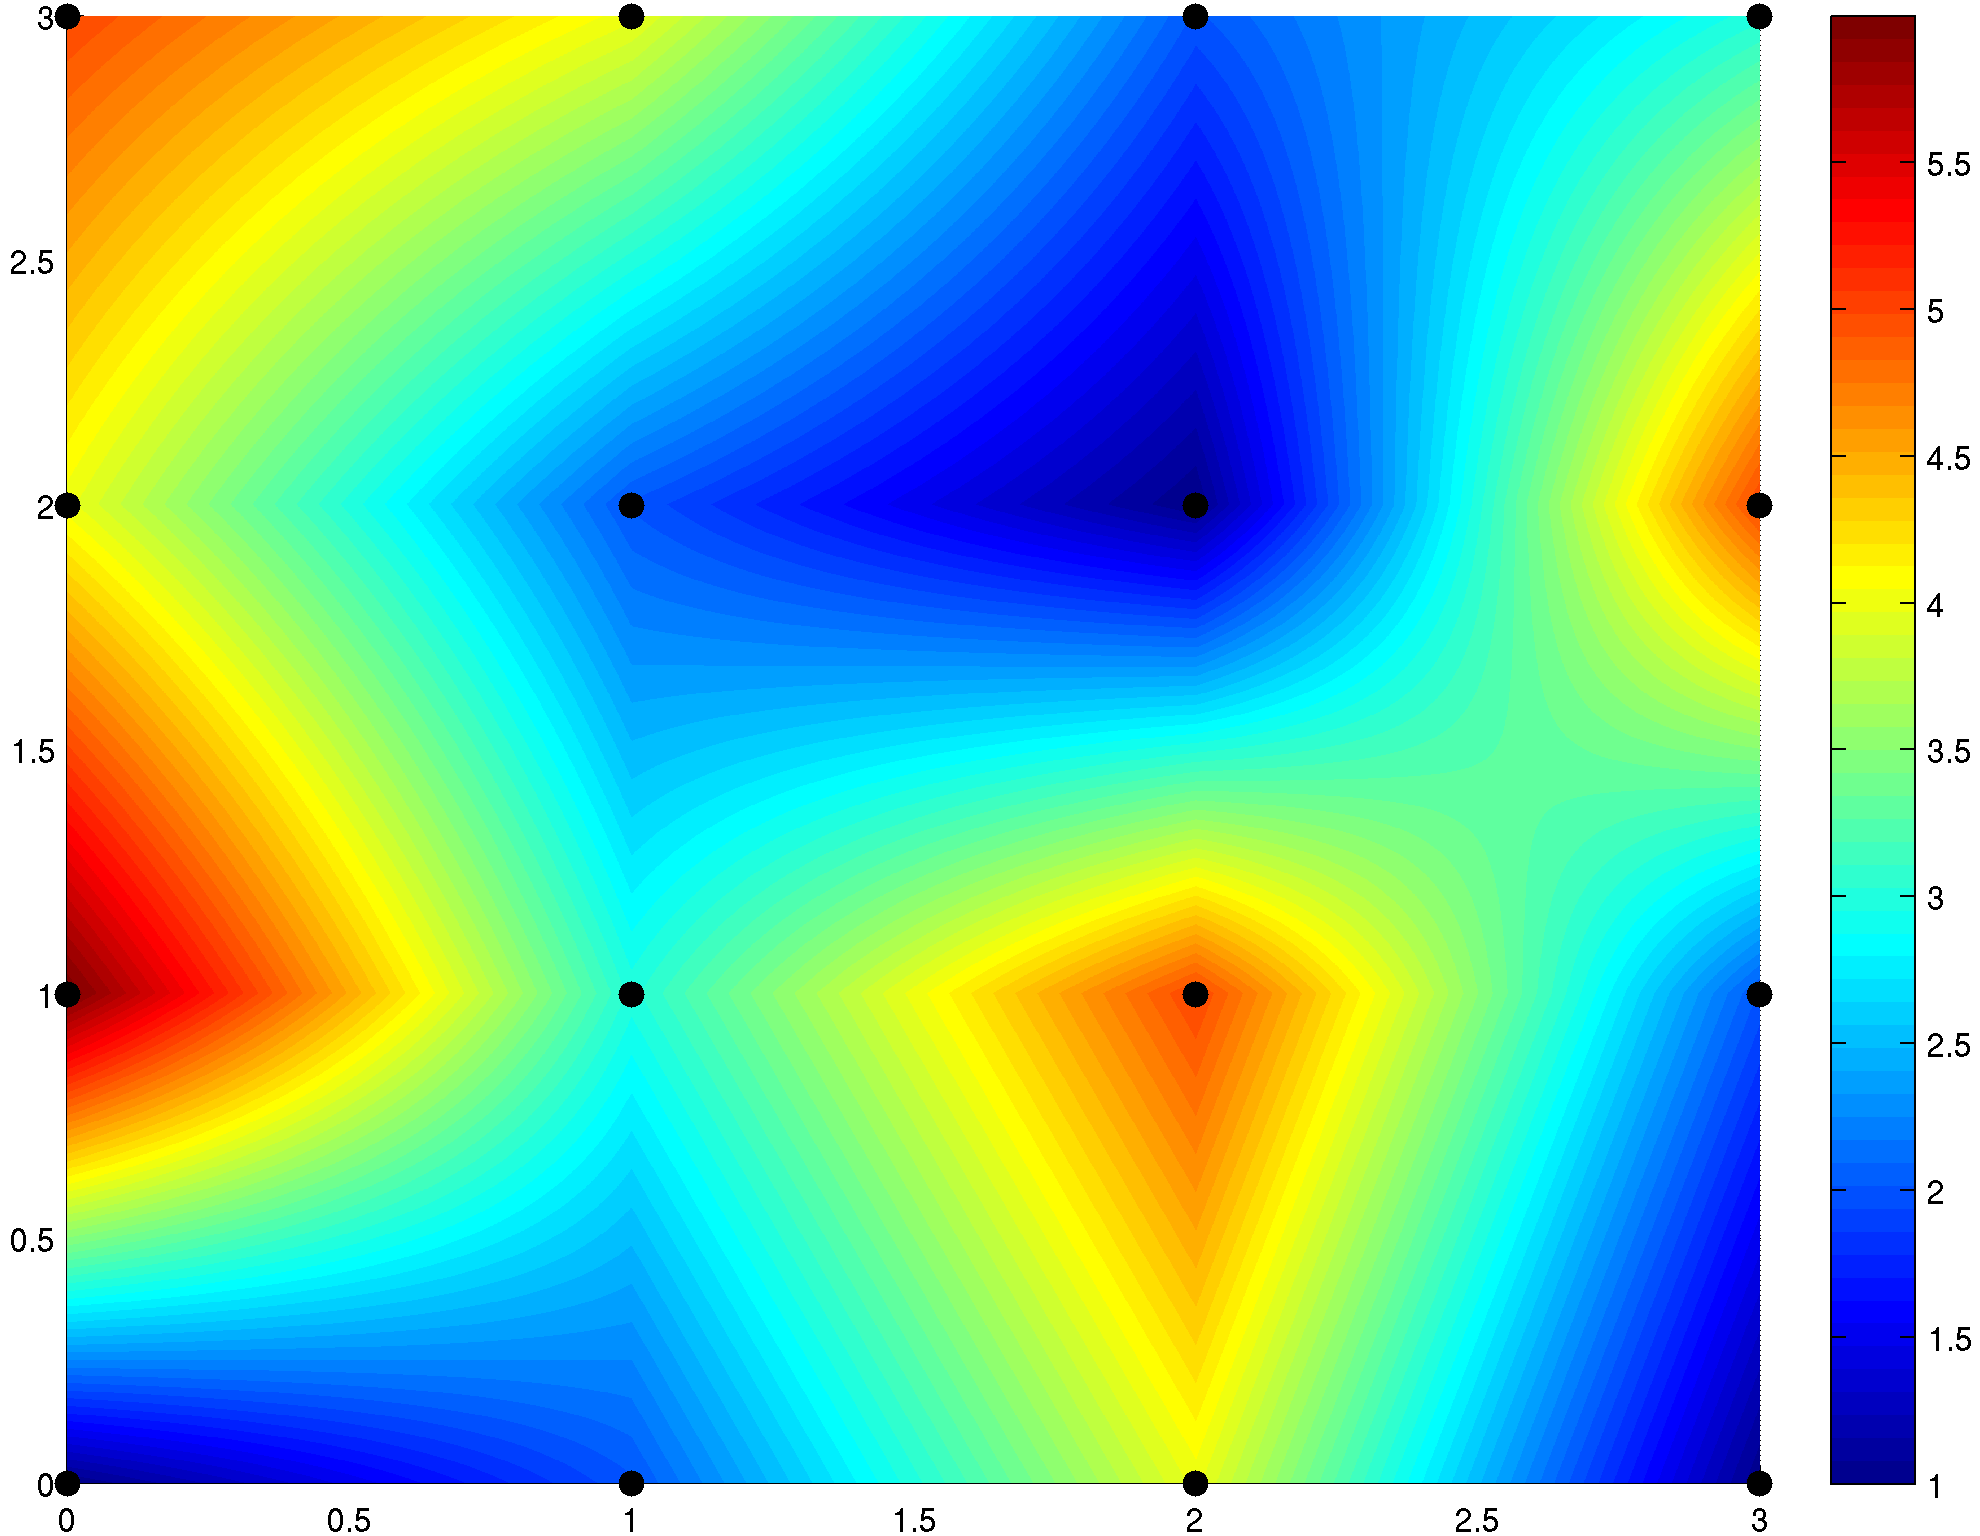
\includegraphics[width=0.9\linewidth]{./images/Bilinear_Interpolation_Example.png}
                    \caption{}
                    \label{fig:example_bilinear}
                \end{subfigure}
                \caption{These examples, created by Wikipedia user \emph{Berland}, shows the difference between bicubic interpolation, figure~\ref{fig:example_bicubic}, and bilinear interpolation, figure~\ref{fig:example_bilinear}, on the same dataset.}
                \label{fig:bicubic_vs_bilinear}
            \end{figure}\mahesh{Should this be in italics?}

            The algorithm for bicubic interpolation is relatively simple, with the result being given by the calculation:

            \begin{align*}
                p(x,y) = \sum_{i=0}^{3}{\sum_{j=0}^{3}{a_{ij}x^{i}y^{j}}}
            \end{align*}

        %\subsubsection{B\'{e}zier Surface}\label{background_interpolation_methods_beziersurface}
        %Probably not since the surface is stretched towards the points, but does not pass through them
        
        %\subsubsection{Lanczos Resampling}\label{background_interpolation_methods_lanczosresampling}
        %Used to interpolate between a sampled signal.
        
        %\subsubsection{Delaunay Triangulation}\label{background_interpolation_methods_delaunaytriangulation}
        %Doesn't give a smooth curve


        \subsubsection{Barnes}\label{background_interpolation_methods_barnes}

            Barnes interpolation uses a multi-pass approach to determine the new data points. The method has found success in calculating air pressure across the United States, providing results similar to careful analysis, however it depends on the data points be reasonably uniform~\cite{barnesinterpolation}.

            No examples existed in either R or Python and so a custom implementation written in Python was created. This implementation follows the information in the original paper by Barnes and has shown success on test data sets. The algorithm works by calculating a simple distance weighted interpolation as the first result, and then iterating multiple times using a calculated error field to reduce the errors in the output. 

            One important factor in Barnes interpolation is the fact that it depends on server constants. These constants depend on the type of data being interpolated and the nature of the measurements, including the density of the measurements. As such, determining these constants is a key part of using this algorithm for interpolation. One advantage of this approach, is that we can iterate over our data set and fit it to the known measurements in order to make sure it is as accurate as possible. With this method however, we lose test data points and so cannot validate it. Experiments using this algorithm have used similar mechanisms and shown success~\cite{pmconcentrationmaps}.

            The algorithm for Barnes interpolation is as follows.

            For the first pass each known point is assigned a weight using the formula: 

            \begin{align*}
                W_{i} &= e^{-(d/R^{2})}
            \end{align*}
            
            where d is the distance between the known point and the current point to be interpolated, and R is the radius of influence. Using this weight, the initial guess of the grid points is calculated as: 
            
            \begin{align*}
                X_{g} &= \frac{\sum_{i}{W_{i}X_{i}}}{\sum_{i}{W_{i}}}
            \end{align*}

            At this point we begin our successive passes. These are defined as:

            \begin{align*}
                X'_{g} &= X_{g} + \frac{\sum_{i}{W'_{i}E_{i}}}{\sum_{i}{W'_{i}}}
            \end{align*}

            where $E_{k}$ is the difference between the estimated value and the actual value at a known point $k$ and $W'_{i}$ is defined as:

            \begin{align*}
                W'_{i} &= e^{-(d/\Gamma R)^{2}}
            \end{align*}

            with $\Gamma$ as a convergence parameter normally set in the range 0.2-0.3.



        
        \subsubsection{Natural Neighbor}\label{background_interpolation_methods_naturalneighbour}
        %Seems like an interesting successor to bicubic
        
        \subsubsection{Spline Interpolation}\label{background_interpolation_methods_splineinterpolation}
        %Basic spline method

    \subsection{Irregular Grid Algorithms}\label{background_interpolation_methods_irregular_grid}

        %\subsubsection{Radial Basis Function}\label{background_interpolation_methods_radial_basis_function}
        %The value will dip between points so probably not what is needed

        %\subsubsection{Thin Plate Spline}\label{background_interpolation_methods_thin_plate_spline}
        %Seems complicated

        %\subsubsection{Least-Squares Spline}\label{background_interpolation_methods_least_squares_spline}
        %A possibility

        %http://en.wikipedia.org/wiki/Nearest-neighbor_interpolation
        \subsubsection{Nearest Neighbour}\label{background_interpolation_methods_nearest_neighbour}

            Nearest neighbour interpolation is the simplest interpolation we will see in that it is not really interpolation at all. Instead the value of each point is the value of the closest data point we have. This algorithm can work reasonably well when there is a small amount of variation. However, as the results it produces are discontinuous, it cannot approximate well when there are large differences between adjacent data points.


        \subsubsection{Inverse Distance Weighting}\label{background_interpolation_methods_inversedistanceweighting}

            The key component of inverse distance weighting (IDW) is the calculation of new parameters as the weighted average of neighbouring parameters. The weighting is calculated as the inverse of the distance from the current point to the neighbour currently being checked and are normalised such that the total weighting is equal to one. Due to the requirement of checking all other points the time complexity of this algorithm, like many other interpolation algorithms, is $O(n^{2})$. However we can reduce this by some constant factor by imposing a maximum radius on all calculations. 

            The general formula for calculating the value, $V$, at a point $X_{i}$ given samples $S$, where $S_{i}$ is the value of sample S, is:

            \begin{align*}
                V = \sum_{i=1}^{N}{
                        \frac{
                            w_{i}(X_{i})S_{i}
                        }{
                            \sum_{j=0}^{N}{w_{j}(X_{j})}
                        }
                    },
            \end{align*}

            where 

            \begin{align*}
                w_{i}(x) = \frac{1}{d(x,S_{i})^{p}}
            \end{align*}

            is a weighting function with $d(X_{1},X_{2})$ being a distance metric between points $X_{1}$ and $X_{2}$, and $p$ is the power parameter, which controls the rate of change at which distances affect the weighting.

            \begin{figure}[H]
                \centering
                \begin{subfigure}{.5\textwidth}
                    \centering
                    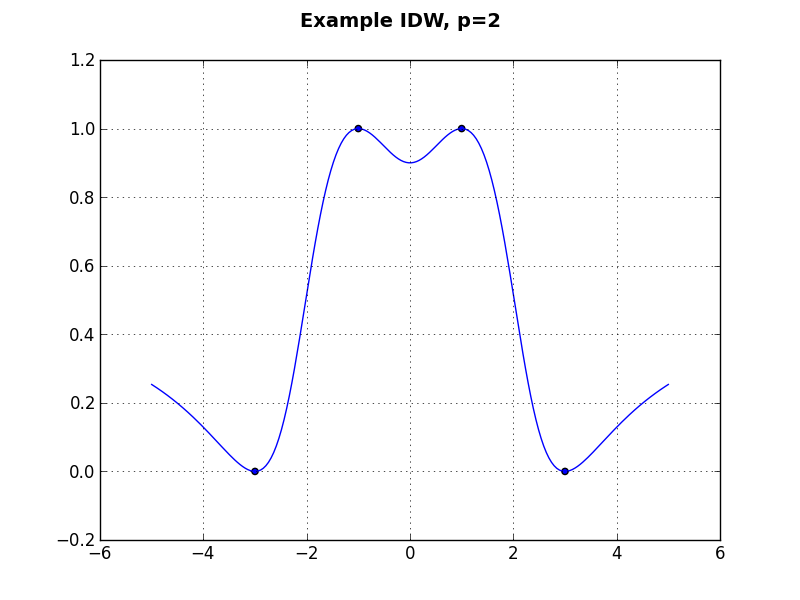
\includegraphics[width=\linewidth]{./images/IDW1.png}
                    \caption{}
                    \label{fig:example_idw_p2}
                \end{subfigure}%DO NOT REMOVE THIS COMMENT
                \begin{subfigure}{.5\textwidth}
                    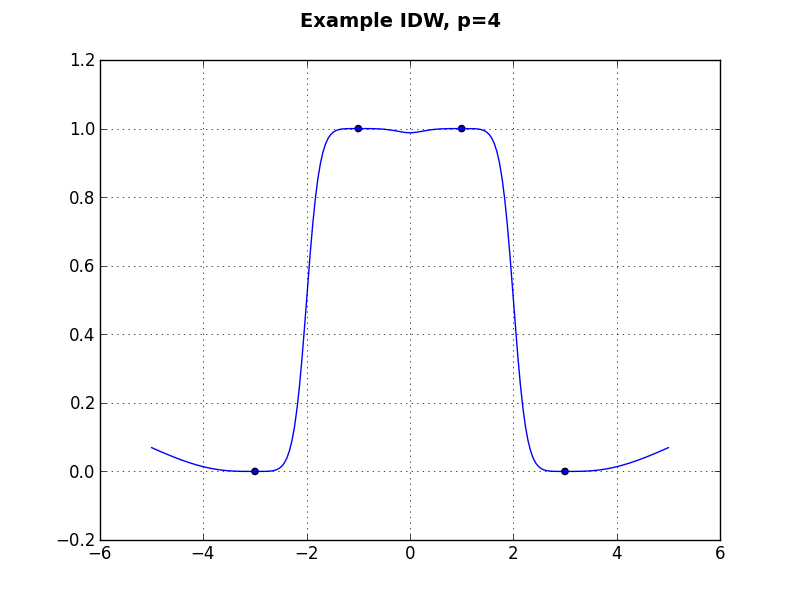
\includegraphics[width=\linewidth]{./images/IDW2.png}
                    \caption{}
                    \label{fig:example_idw_p4}
                \end{subfigure}
                \caption{These two figures show the IDW algorithm in one dimension at points -3,-1,1 and 3 where the values are 0,1,1 and 0 respectively. Figure~\ref{fig:example_idw_p2} has a power parameter of 2, while figure~\ref{fig:example_idw_p4} has a power parameter of 4.  }
                \label{fig:example_idw}
            \end{figure}

            As we can see in figure~\ref{fig:example_idw} IDW's dependence on the surrounding values causes interesting effects. Between the x values of -1 and 1 we can see a local minima in the graph. This is due to the fact that the values at -3 and 3 are lower and are taken into account. Should these values be further away, such as we see in figure~\ref{fig:example_idw_distance}, the effect is less pronounced. A further way of mitigating this effect is to increase the power parameter as has been done in figure~\ref{fig:example_idw_p4}. It should be noted, however, that as the p factor goes to infinity, the IDW algorithm approaches the nearest neighbour algorithm. 

            \centerimage{.5\textwidth}{./images/IDW3.png}{In this figure the two extreme points have been moved further from zero by a value of one, in order to demonstrate their effect on the value at zero decreasing compared to figure~\ref{fig:example_idw_p2}}{fig:example_idw_distance}
        %\subsubsection{Kriging}\label{background_interpolation_methods_kriging}
        % Very complicated and requires a lot of domain specific knowledge
